\documentclass[10pt,letterpaper]{article}
\usepackage[margin=0.78in]{geometry}
\usepackage[T1]{fontenc}
\usepackage{lmodern,microtype,graphicx,booktabs,tabularx,amsmath,xcolor,enumitem,fancyhdr}
\usepackage[hyphens]{url}
\usepackage[colorlinks=true,linkcolor=teal,urlcolor=teal]{hyperref}
\definecolor{ink}{HTML}{243447}
\definecolor{teal}{HTML}{006B72}
\setlength{\parindent}{0pt}\setlength{\parskip}{6pt}
\setlist{nosep,leftmargin=1.5em}
\pagestyle{fancy}\fancyhf{}\fancyhead[L]{\small Product counts and recall-event counts}\fancyhead[R]{\small Independent study 17}\fancyfoot[C]{\thepage}
\setlength{\headheight}{14pt}
\hypersetup{pdftitle={Product counts and recall-event counts},pdfauthor={Independent research program},pdfsubject={Retrospective administrative counting comparison; not public alerts or medical advice}}
\begin{document}\color{ink}
{\LARGE\bfseries Product counts and recall-event counts\par}
{\large How counting units change a fixed research-review queue\par}
\textbf{Independent research study 17}\hfill 29 October 2026\\
AI-assisted analysis and manuscript. Not peer reviewed or accepted for formal publication.

\section*{Decision and verified finding}
An internal data-review queue needs a clear unit of work. FDA assigns a recall number to a classified product and an event ID to a recall event; one event can contain several products. Product rows are useful detail. They are not interchangeable with event counts, and products under one event are not automatically duplicate errors.

We retained all 16,324 food enforcement product records reported during 2017--2025 in the captured openFDA snapshot. The fixed 2022--2025 evaluation contains 6,833 products and 1,954 distinct event IDs. Applying a calibration-derived event threshold to product counts flags 41 of 48 evaluation months; applying it to event counts flags one. This large contrast exposes a unit mismatch. With a separate product threshold, each counting policy flags one month, but they flag different months.

\begin{center}\begin{tabularx}{\linewidth}{Xrr}\toprule
95th-percentile policy & Threshold & Flagged months\\\midrule
Events against event threshold & 71.15 events & 1 / 48\\
Products against event threshold & 71.15 (mismatched unit) & 41 / 48\\
Products against product threshold & 453.20 products & 1 / 48\\\bottomrule
\end{tabularx}\end{center}

\textbf{Practical recommendation.} Keep a lossless product table and an explicit event view. Choose whether a review task concerns product-detail workload or distinct events, and calibrate its threshold in that same unit. Preserve links back to every product when grouping events. Matching aggregate flag counts is insufficient: inspect which months each policy selects.

\textbf{Limits.} This is a retrospective administrative snapshot, not a public recall-alert system, medical decision tool or reconstruction of amendment history. FDA warns against using this endpoint for public alerts or recall-lifecycle tracking. We do not measure true safety incidents, missed hazards, false alarms, labor savings or future performance. The illustrative quantiles are fixed policy conventions, not optimized detectors.

\textbf{Scientific contribution.} A reproducible comparison with complete grain, threshold and sensitivity accounting, using established counting and quantile methods. A bounded primary-source review does not establish scientific novelty. The broader original proposal's human-audited labels, amendment lineage and prospective alert evaluation are not claimed.

\clearpage
\section*{1. Source, rights and observation unit}
The openFDA food enforcement API serves publicly releasable FDA Recall Enterprise System data and is normally updated weekly [1]. We requested each report-date year from 2017 through 2025, sorting the exact recall-number field ascending, with pages of up to 1,000 records. Retrieval captured 21 pages; nine final count probes matched initial annual totals and the common metadata version, 2026-10-21. Requests, timestamps and raw/subset SHA-256 hashes are retained. Consistent metadata and counts are bounded retrieval evidence, not a transactional atomic-snapshot guarantee.

Only five source fields are published: recall number, event ID, report date, classification and product type, with year/page/row locators. Complete original responses stay outside Git. No firm/address, narrative, precise location, adverse-event/patient or device/GMDN data is included. The selected food administrative fields fall under openFDA's public-domain/CC0 default, subject to its stated exceptions; attribution implies no FDA endorsement [5].

\begin{center}\begin{tabular}{rrl}\toprule
Report year & Product records & Partition\\\midrule
2017 & 3,203 & Calibration \\
2018 & 1,958 & Calibration \\
2019 & 1,863 & Calibration \\
2020 & 1,286 & Calibration \\
2021 & 1,181 & Calibration \\
2022 & 1,652 & Evaluation \\
2023 & 2,155 & Evaluation \\
2024 & 1,409 & Evaluation \\
2025 & 1,617 & Evaluation \\
\bottomrule\end{tabular}\end{center}

All records passed the unchanged nonempty-field, valid date/year, positive event-ID, unique recall-number, Food-only and three-class gates. All 108 months contain products/events. Each class has at least 20 nonzero calibration months: Class I and II each have 60; Class III has 56. Exact selected and normalized source-field checks total 261,184. No source row was discarded to meet an outcome-dependent criterion.

\begin{center}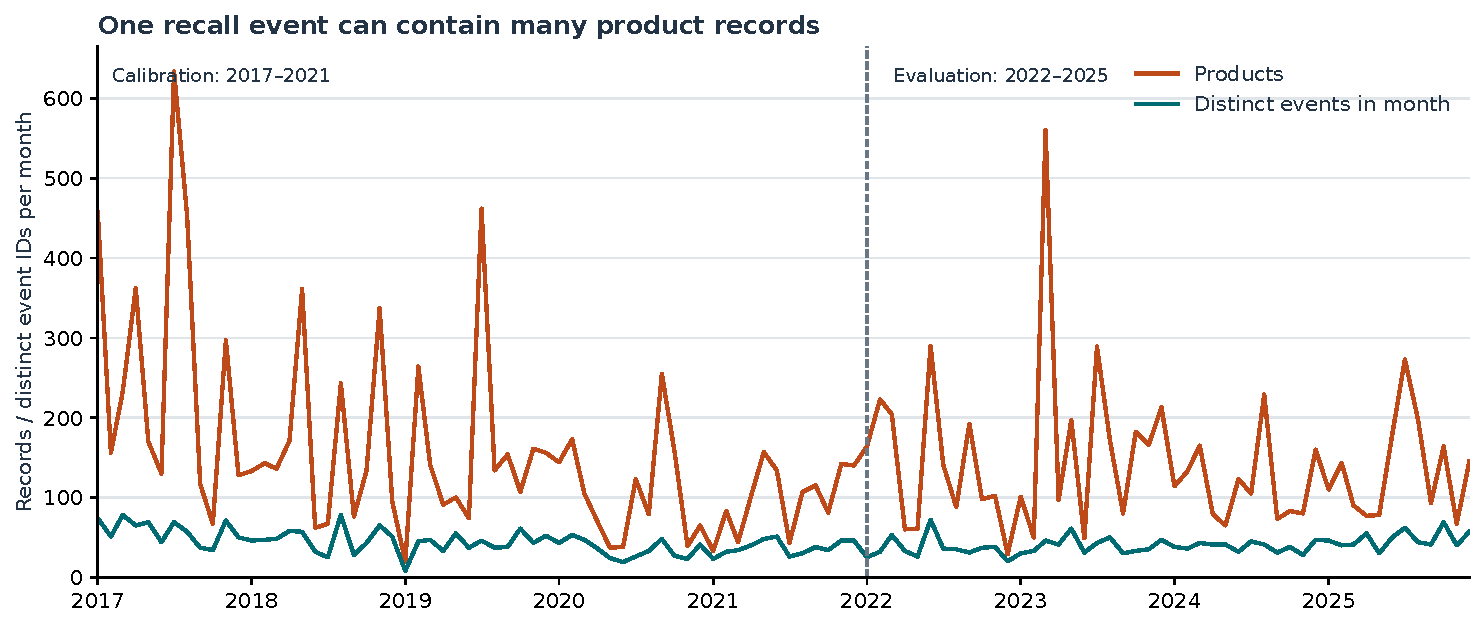
\includegraphics[width=\linewidth]{images/monthly-counts.pdf}\end{center}
\textbf{Figure 1.} All-class monthly product records and distinct event IDs. The dashed line marks the fixed report-date split. Both series start at zero on the same count scale. Monthly event counts are an administrative grain, not population risk or true new-incidence counts.

\clearpage
\section*{2. Fixed protocol and comparison}
FDA's product/event definitions govern entity semantics [2]. For panel $c$ and report month $m$, $P_{cm}$ is the product-row count, $U_{cm}$ the distinct recall-number count and $E_{cm}$ the distinct event-ID count. The uniqueness gate requires $P_{cm}=U_{cm}$. Products remain intact. Fanout is $P_{cm}/E_{cm}$ when $E_{cm}>0$; a zero-event secondary cell is encoded as zero for tabulation, with both counts available. Excess $P-E$ measures a grain difference, not erroneous duplication or avoidable work.

The primary panel includes all food records. Three secondary panels use FDA classes. An event may include products in more than one class, so class-event counts must not be added to obtain the all-class event count. Events are counted within each month; no cross-month removal, status model or first-publication inference is used.

\subsection*{Thresholds and protected evaluation}
Calibration uses the 60 months of 2017--2021. Evaluation uses the 48 months of 2022--2025. Before evaluation event counts, fanout or flags were computed, code, source and 64 thresholds were committed and twelve dependencies hashed in a public freeze. Only all-year source format/coverage counts were inspected earlier. Development SQL explicitly excludes evaluation years before aggregation. These are partitions of a later snapshot; the split does not recover what was known at each historical date.

For sorted calibration counts $x_{(0)},\ldots,x_{(n-1)}$, use the fixed type-7 linear quantile:
\[
h=(n-1)q,\quad i=\lfloor h\rfloor,\quad
Q_q=x_{(i)}+(h-i)(x_{(\min(i+1,n-1))}-x_{(i)}).
\]
The primary $q=0.95$ and sensitivities $q=0.90,0.99$ were prespecified. A flag requires count strictly greater than its threshold; equality is not flagged. Thresholds are exact rational numbers. There is no tuning, fitted model, seed or hyperparameter search. These conventions are illustrative; they are not calibrated against verified hazard labels or a stated operational service level.

\begin{center}\begin{tabular}{lrr}\toprule
Panel & Event threshold & Product threshold\\\midrule
All & 71.15 & 453.20 \\
Class I & 34.20 & 157.30 \\
Class II & 37.10 & 263.70 \\
Class III & 7.00 & 24.80 \\
\bottomrule\end{tabular}\end{center}
\textbf{Table 1.} Primary 95th-percentile thresholds, in events/month and products/month respectively. No class weighting or optimization was performed.

We retain three policies: events against their event threshold; products against that same event threshold (a deliberately mismatched comparator); and products against a separately calibrated product threshold (the fair comparator). Every panel/quantile/policy month is retained. For the primary quantile, each calibration year is also omitted in turn, recalibrating on 48 months and keeping the evaluation period fixed. No result selects a preferred threshold.

\clearpage
\section*{3. All-class results and multiplicity}
Calibration contains 9,491 products and 2,647 event-months, or 3.59 products per event-month. Evaluation contains 6,833 products and 1,954 event-months, or 3.50. Across the complete snapshot there are 4,601 distinct event IDs. No event ID spans more than one report month in this capture; that observed fact is not a guarantee for other exports. Ninety-eight event IDs include multiple classes (51 calibration, 47 evaluation), illustrating why class-event totals can overlap.

The largest evaluation monthly fanout is March 2023: 560 products over 46 events, or 12.17 products per event-month. Its largest event accounts for 409 products; the five largest account for 85.5\% of the month's products. This concentration is compatible with many legitimate product entries within one event. The data do not identify whether any row is an erroneous duplicate or whether later amendments caused the concentration.

\begin{center}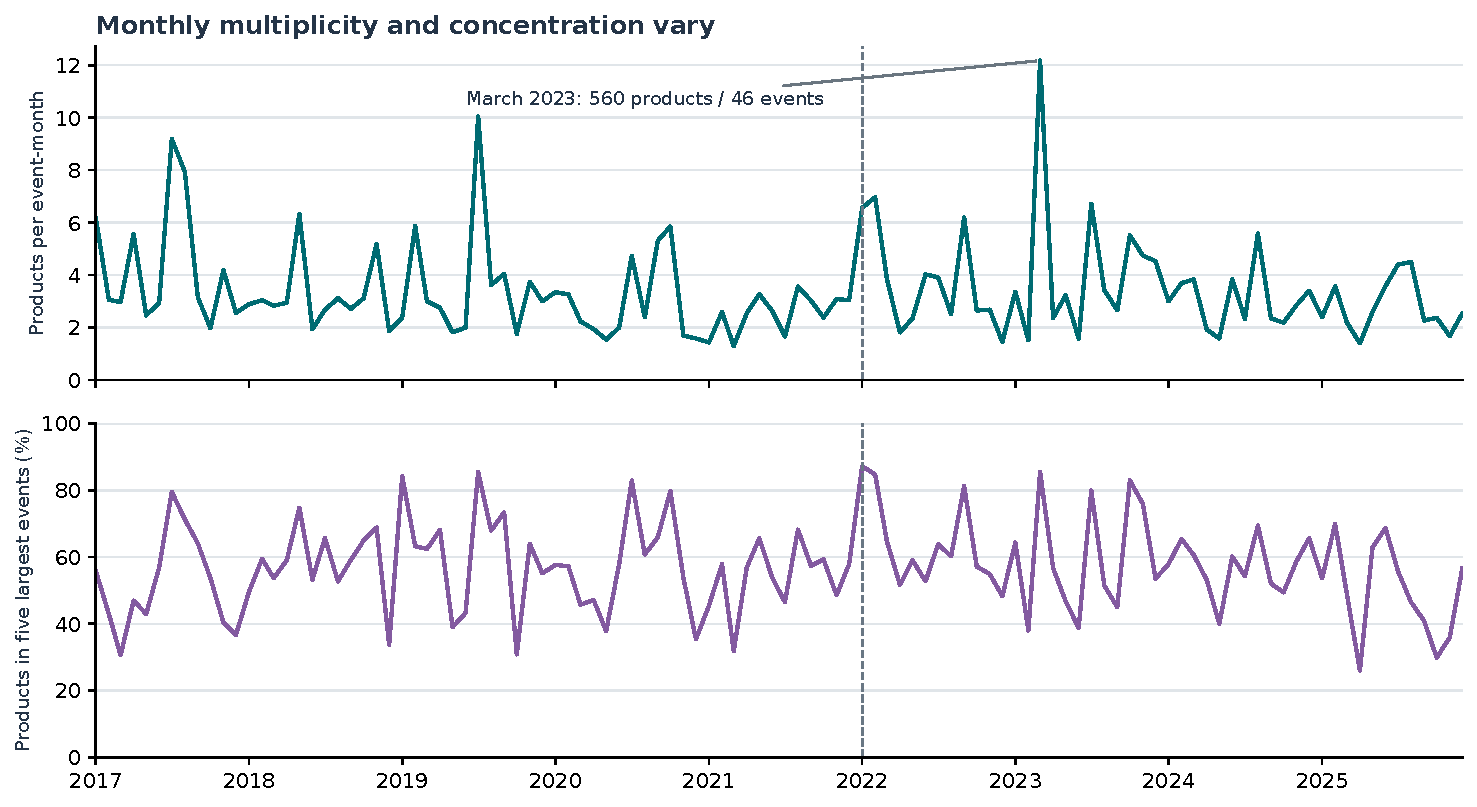
\includegraphics[width=\linewidth]{images/event-fanout.pdf}\end{center}
\textbf{Figure 2.} All-class within-month multiplicity and product concentration. Top: products per event-month. Bottom: fraction of products in the five largest event groups, expressed as a percentage. Separate axes have explicit units and start at zero. The dashed line marks evaluation. No uncertainty band is drawn because these are exact counts of the captured finite snapshot, not estimates from a sample of its rows.

At the primary quantile, event counts flag June 2022. The separately calibrated product policy flags March 2023. They agree on 46 unflagged months and have no jointly flagged month. Thus a matched total of one flag per policy conceals a different review focus. Neither policy is treated as ground truth.

\clearpage
\section*{4. Policy agreement and secondary panels}
The primary mismatch comparison yields 40 product-policy-only months, one shared flag, zero event-only months and seven months flagged by neither. The own-threshold comparison yields one product-only month, one event-only month, zero shared flags and 46 months flagged by neither. These are policy discordances, not false-positive or false-negative estimates.

\begin{center}\small\begin{tabular}{lrrrrrr}\toprule
Quantile & E flags & P same & P own & Both own & P-only own & E-only own\\\midrule
90th & 2 & 42 & 1 & 0 & 1 & 2 \\
95th & 1 & 41 & 1 & 0 & 1 & 1 \\
99th & 0 & 38 & 1 & 0 & 1 & 0 \\
\bottomrule\end{tabular}\end{center}
\textbf{Table 2.} All-class evaluation, 48 months. P same uses the event threshold; P own uses the product threshold. Both/P-only/E-only refer to the fair own-threshold comparison against the event policy. The full contingency tables retain months flagged by neither.

\begin{center}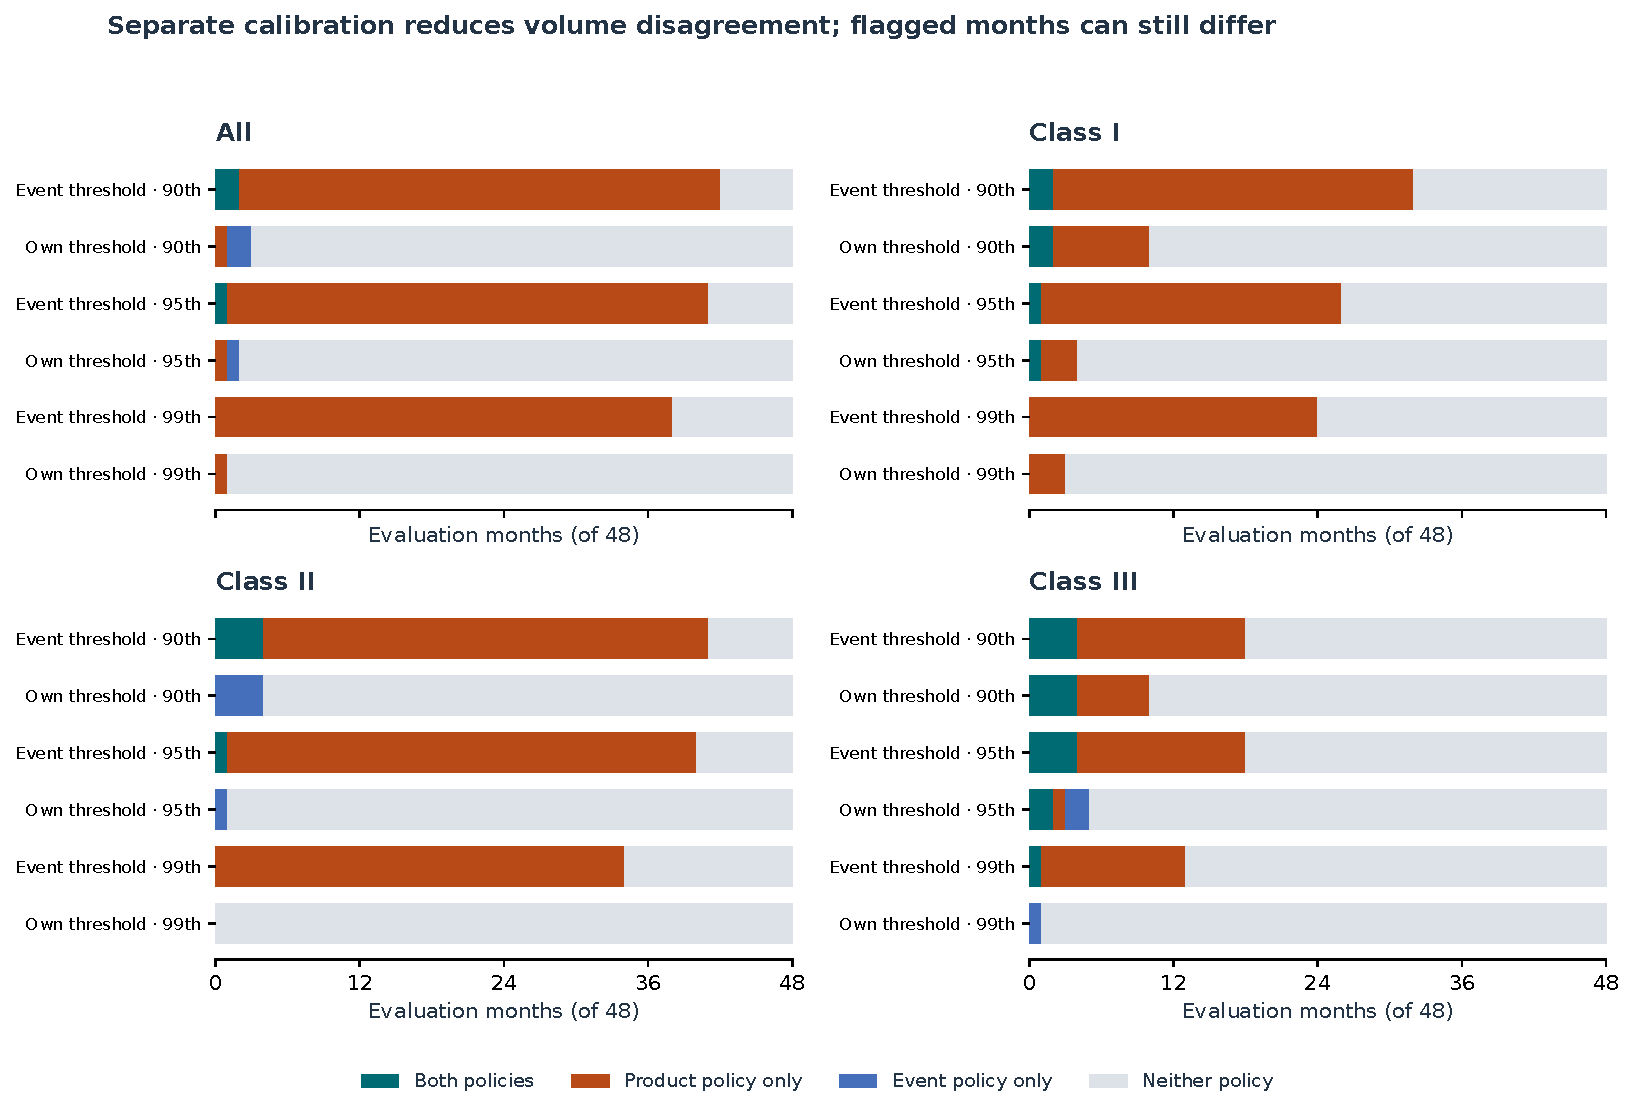
\includegraphics[width=\linewidth]{images/flag-agreement.pdf}\end{center}
\textbf{Figure 3.} All evaluation-month agreements for four panels, three fixed quantiles and both product-threshold choices. Each bar totals 48 months. Event threshold labels denote the product policy using that event threshold; own threshold denotes separate product calibration. Colors describe agreement only, not verified safety outcomes. Class panels can overlap in event membership and should not be summed.

\clearpage
\section*{5. Sensitivity, implications and limits}
\begin{center}\small\begin{tabular}{lrrrrrr}\toprule
95th-percentile panel & E flags & P same & P own & Both own & P-only own & E-only own\\\midrule
All & 1 & 41 & 1 & 0 & 1 & 1 \\
Class I & 1 & 26 & 4 & 1 & 3 & 0 \\
Class II & 1 & 40 & 0 & 0 & 0 & 1 \\
Class III & 4 & 18 & 3 & 2 & 1 & 2 \\
\bottomrule\end{tabular}\end{center}
\textbf{Table 3.} Secondary class results under the primary quantile, with all-class context. They are descriptive comparisons, not separate discoveries selected for significance. With separate calibration, Class I flags four product months versus one event month; Class II flags zero versus one; Class III flags three versus four. A fair baseline narrows the broad mismatch contrast but does not make the units interchangeable.

\begin{center}\small\begin{tabular}{lrrrrrr}\toprule
Omitted cal. year & E flags & P same & P own & Both own & P-only own & E-only own\\\midrule
2017 & 4 & 45 & 1 & 0 & 1 & 4 \\
2018 & 1 & 41 & 1 & 0 & 1 & 1 \\
2019 & 0 & 41 & 1 & 0 & 1 & 0 \\
2020 & 0 & 41 & 1 & 0 & 1 & 0 \\
2021 & 0 & 41 & 1 & 0 & 1 & 0 \\
\bottomrule\end{tabular}\end{center}
\textbf{Table 4.} All five prespecified calibration-year omissions, all-class primary quantile. Evaluation remains fixed. Event flags range from zero to four, same-threshold product flags from 41 to 45, and own-threshold product flags remain one. These finite sensitivity ranges are not confidence intervals. No omitted-year result is selected to replace the primary threshold.

\textbf{Use the counting unit that matches the review question.} An event view can help examine distinct regulatory groupings; a product view can help inspect product-specific detail. Retain both, name the denominator in charts and export formats, and document calibration units alongside every threshold. A prospective internal operational evaluation would need verified queue actions, actual staff time and historical data availability before any efficiency or performance claim.

\textbf{Material limitations.} FDA may correct records or expand recalls after the original report. One current export contains no reliable amendment history, complete lifecycle sequence or historical information vintages [1]. Report dates are not assumed to be recall initiation, public warning or first API availability. Food categories, firms and exposure are outside this minimized panel. Publicly releasable classified records do not establish complete underlying hazards or consumer exposure. The selected quantiles have no validated safety objective. Month-to-month dependence and structural change may matter operationally; no inferential coverage or future false-alarm guarantee is claimed. Exact grouping does not validate FDA's entity assignments. No human-audited linkage sample, NLP model, deployed service, peer review or novel method is asserted.

\clearpage
\section*{6. Reproduction and independent evidence}
\begin{tabularx}{\linewidth}{lX}\toprule
Check & Actual evidence\\\midrule
Boundaries & Nine fixtures cover product preservation, month/class overlap, quantile interpolation/equality, matched units, duplicate IDs, gaps and unknown labels.\\
Source & All 261,184 selected/normalized fields checked; 21 pages and nine final count/version probes reconciled. Full originals remain outside Git.\\
Development & 13,608 independent values; no floating difference in retained ratios.\\
Evaluation & 10,685 independent values; no floating difference in retained ratios.\\
Replay & 196,440 exact fields or JSON documents and 1,296 floating fields rebuilt offline from the minimized source; twelve frozen dependencies verified.\\
Figures & All 528 plotted values independently checked with SQL, rational ratios and verified policy flags. Three original figures; every manuscript page rendered for inspection.\\\bottomrule
\end{tabularx}

SQLite independently reconstructs distinct counts and memberships; decimal interpolation reconstructs all rational thresholds; Fraction arithmetic checks concentrations and comparisons. Separate contingency histograms check every agreement table. Integers, thresholds and flags require exact equality; the stated absolute tolerance for reported floating ratios is $10^{-12}$. The current checks returned zero ratio difference. Finite successful checks are not universal correctness, privacy or accessibility certification.

From a clean checkout with Python 3.10, install the pinned requirements and run:
\begin{verbatim}
python -m pip install -r requirements.txt
python -m unittest discover -s tests -v
python src/check_reproduction.py
python src/verify_figures.py
python src/verify_paper.py
python src/verify_public_package.py
\end{verbatim}
Public replay does not require a live API or the excluded full responses. The source verification certificate records the earlier complete original-to-subset check. Package checking binds reviewed canonical Git blobs and five explicitly approved independent manuscript files. Formal-publication projects, including Azure optimization, remain private. Remote release proof is maintained in the program register after exact-head Linux, tested/merged-tree and annotated-tag verification; it is not inferred from a local test.

\section*{Primary references}
\small
[1] FDA, \href{https://open.fda.gov/apis/food/enforcement/}{Food enforcement overview}. Weekly RES data, later corrections/expansions, public-alert/lifecycle restrictions. Accessed 29 October 2026.\par
[2] FDA, \href{https://www.fda.gov/safety/enforcement-reports/enforcement-report-information-and-definitions}{Enforcement Report information and definitions}. Product and event views; identifier meanings.\par
[3] openFDA, \href{https://open.fda.gov/apis/food/enforcement/searchable-fields/}{Food searchable fields} and \href{https://open.fda.gov/apis/query-parameters/}{query parameters}. The food page's linked shared YAML resolves to a drug-enforcement schema; FDA definitions in [2] govern semantics here.\par
[4] Kass-Hout et al. (2016). OpenFDA: an innovative platform providing access to a wealth of FDA's publicly available data. \emph{JAMIA} 23:596--600. \href{https://doi.org/10.1093/jamia/ocv153}{doi:10.1093/jamia/ocv153}. Platform context only.\par
[5] openFDA, \href{https://open.fda.gov/license/}{Data licensing} and \href{https://open.fda.gov/terms/}{terms}. CC0 default and stated exceptions; no endorsement.
\end{document}
